\documentclass[DM,authoryear,toc]{lsstdoc}
% lsstdoc documentation: https://lsst-texmf.lsst.io/lsstdoc.html
\input{meta}

% Package imports go here.

% Local commands go here.

%If you want glossaries
%\input{aglossary.tex}
%\makeglossaries

%\title{Lightweight Alert Packets}
\title{A Hybrid Notification and Alert Retrieval Service}

% Optional subtitle
% \setDocSubtitle{A subtitle}

\author{%
Eric Bellm,
Spencer Nelson
}

\setDocRef{DMTN-165}
\setDocUpstreamLocation{\url{https://github.com/lsst-dm/dmtn-165}}

\date{\vcsDate}

% Optional: name of the document's curator
% \setDocCurator{The Curator of this Document}

\setDocAbstract{%
We consider the implications of providing a subset of alert packet contents in the alert stream, with the full alert packets available for rate-limited retrieval using an identifier included in the ``lightweight'' alert.
This hybrid approach would enable much wider dissemination of the complete lightweight alert stream, potentially to thousands more users than is possible in the current baseline.
In turn this ``alerts on your laptop'' access would allow users to conduct more sophisticated filtering and analysis than the current Alert Filtering Service, increasing the overall scientific returns of the alert stream.
Community brokers would still be able to retrieve all of the contents of the full alert stream within the 60 second latency window and would gain greater control over their ingestion of the bulk alert data.
Technically, this hybrid system may represent a modest increase in complexity over the current baseline but is likely to be more operationally robust.
}

% Change history defined here.
% Order: oldest first.
% Fields: VERSION, DATE, DESCRIPTION, OWNER NAME.
% See LPM-51 for version number policy.
\setDocChangeRecord{%
  \addtohist{1}{YYYY-MM-DD}{Unreleased.}{Eric Bellm}
}


\begin{document}

% Create the title page.
\maketitle
% Frequently for a technote we do not want a title page  uncomment this to remove the title page and changelog.
% use \mkshorttitle to remove the extra pages

% ADD CONTENT HERE
% You can also use the \input command to include several content files.

\section{Background}

As it conducts the Legacy Survey of Space and Time, the Rubin Observatory will produce a near-real-time alert stream to notify astronomers around the world of all the transients, variables, and moving objects that it detects in difference imaging.
Rubin Observatory alerts are immediately world-public and are intended to facilitate timely follow-up of time-critical events.
Alerts are sent to third-party community brokers for further enhancement and redistribution and are also available to Data Rights holders through the Alert Filtering Service.

In order to provide all of the information needed to make rapid classification and follow-up decisions, the alert packets are ``rich''--they contain not only the information about the latest detection, but also past detection history, forced photometry and/or upper limits, the associated \DIAObject or \SSObject record, linkages to counterparts in the most recent LSST data release, and image cutouts.
The alert contents are public and freely shareable \citedsp{RDO-013}.

Because of the large amount of data in each alert, the alert packets are relatively large.
\citeds{DMTN-102} aggregates relevant sizing information about alerts.
Alert sizes of 82\,KB have been estimated from simulations, although since the image cutouts are sized with the detection footprint\dmreq{0274}, packet sizes of a few megabytes have been seen in processing of precursor data.
To send 10,000 alerts of 82\,KB within a nominal 5-second window of the allowed 60-second alert latency, more than 1 Gbps of outbound bandwidth is required.  
This constraint in turn limits the number of community alert brokers that can be supported; a minimum of five brokers is required\dmreq{0391}.
Accordingly Rubin Observatory is conducting a proposal process to select which community brokers will be allowed to directly receive the full alert stream.

\citeds{DMTN-093} describes the baseline technical design for the Rubin Observatory Alert Distribution System.
Alerts are serialized to a strongly-schemaed binary format, Apache Avro, for compactness.
The open-source distributed streaming platform Apache Kafka provides the alert distribution interface---selected community brokers will connect to the Rubin Kafka cluster and consume the alert stream via Kafka clients.
This approach has been demonstrated at smaller scale by the Zwicky Transient Facility \citep{Patterson:19:ZTFAlertDistribution}.


\begin{figure}
  \begin{centering}
  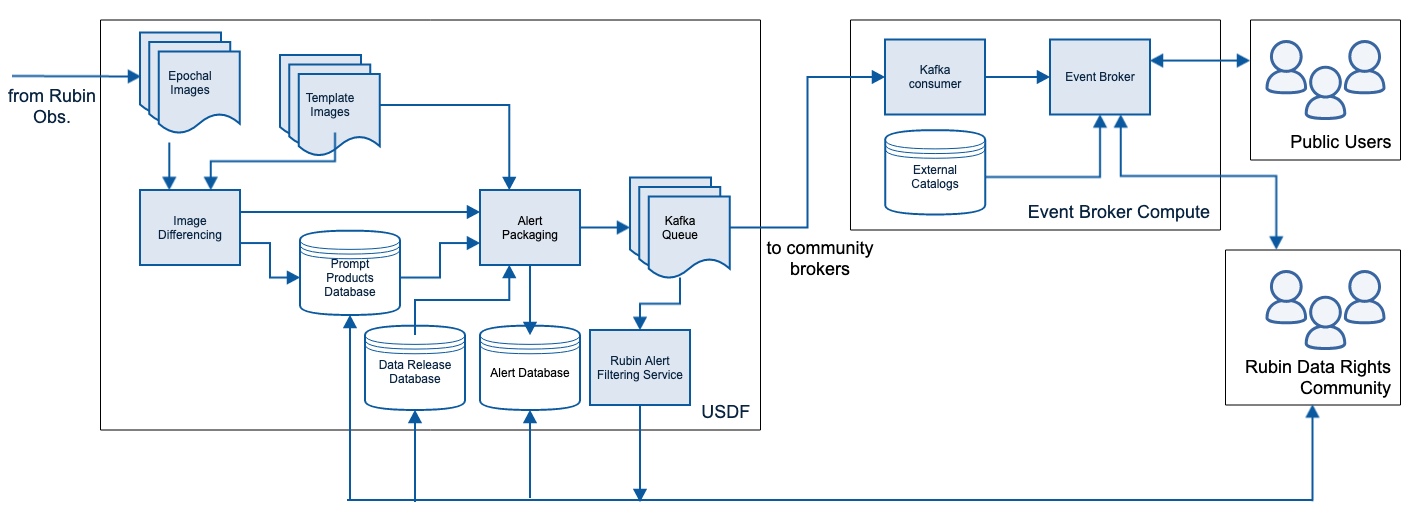
\includegraphics[width=\textwidth]{fig/baseline_alert_dist.png}
  \caption{Data flow diagram for the baselined Alert Distribution System. 
  \label{fig:baseline}}
  \end{centering}
\end{figure}


\section{Motivation}

The large size of the alert packet in the baseline design creates several problems.
Most importantly, it makes outbound bandwidth from the Data Facility the primary constraint on the system.
As a result, only a small number of consumers can receive the full alert stream.
This limits the reach and impact of the alert stream and hinders the flexibility and creativity of scientists.
Moreover, both brokers and users must stream through each large packet on their system, even if they intend to filter it out and discard it---this makes handling the alert stream more technically challenging than is necessary.
Because of the requirement to send alerts to brokers within 60 seconds of readout, outbound bandwidth usage is extremely ``peaky''--most of the traffic is sent within $\sim$5 seconds of every 39 seconds.
Finally, Kafka, the baselined technology for alert distribution, is optimized for small messages ($\sim$1\,kB\footnote{\url{https://docs.cloudera.com/documentation/kafka/latest/topics/kafka_performance.html}}), and performance can degrade as message size increases.
The large range of alert packet size due to variable-size cutouts poses a particular challenge in this regard as we must configure a maximum message size for Kafka.
While these implementation details are specific to Kafka, they reflect a current architectural design consensus within the software community that notification should be separated from data delivery.
It is difficult to build a system that simultaneously provides rapid, reliable notifications as well as efficient delivery of bulk data!
%  Problems with the baseline:
%    (tech antipattern, per Chris M)
%    Large alert stream limits audience
%    Users have to handle entire packet
%    Peaky usage of bandwidth
%    Kafka doesn't like large messages

Our overarching goal for considering a hybrid alert architecture is the enhance the scientific return of the LSST alert stream by ensuring a large and robust broker and user ecosystem and by improving performance and access for individual users relative to the baseline.
At the 2019 community broker workshop, there was clear consensus among the attendees that the Project should explore avenues that would broaden access to the alert stream.
At the same time we want to maintain the rich content of the alert packet to enable rapid filtering and analysis and enable the alerts to be widely shared publicly.

  %Goals:
  %  (cite broker workshop)
%    enhance scientific return of LSST alert stream.  improve performance and access for individual users, enable a large broker and user ecosysystem

\section{The Hybrid Alert Packet Concept}

Before describing the hybrid alert concept, we first stress that we are not advocating for a change to the relevant requirements\lsrreq{0101}\reqparam{OTT1}\dmreq{0391}\reqparam{numStreams}\dmreq{0274}.
We will still produce all of the required alert contents and be capable of transmitting them to the required number of brokers within the required 60 second window after readout completes.

In the hybrid alert packet concept, the realtime alert stream still contains information about all detection \DIASources.
However, the transmitted packets contain much less information than the full alert packets described in the DPDD.
This lightweight ``notification stream'' would contain a bare minimum of science data to allow users to determine a subset of alerts that are of potential interest and retrieve the full packets only for those alerts.
We expect that many science use cases will only require retrieval of a few percent or less of the corresponding full alerts. 

Appendix \ref{sec:lightweight_contents} provides a draft set of potential lightweight alert contents.
They are not meant to completely characterize any event, but merely to provide maximum scientific distinguishing power, to allow users to determine if this alert is likely a transient, variable, or moving object.
It is expected that users will still need to retrieve the full alert packet to be able to achieve their science goals.

The size of the lightweight alert is $\sim$200 bytes/packet. 
Averaged over 39 seconds per visit this implies an average bandwidth required of 400 kbps; to transmit all of the lightweight alerts in a visit within 5 seconds requires 3.2 Mbps.
This implies that we can easily serve thousands of users the lightweight alert stream using a 10 Gbps network interface from the Data Facility.
A night of observing would produce a total volume of lightweight alerts of 2\,GB.
In contrast to the full alert stream, which is $\sim$ 820\,GB per night, it is easy to imagine a graduate student accessing the full alert stream from their laptop, or perhaps connecting a small or ad-hoc automated telescope to it.
We believe that democratizing access to the alert stream will enable some of the most creative uses of the stream and ensure innovative use by scientists.

Each lightweight alert packet would include a link to allow the user to retrieve the full alert packet containing all of the DPDD-specified quantities (image cutouts, \DIASource history, forced photometry where available, timeseries features, etc.).
Rate limits assigned to each user would manage bandwidth use.
The typical workflow will be for users to inspect the contents of the lightweight alert, filter them down to a relevant subset (e.g., alerts coincident with the LMC; alerts in deep drilling fields; fast-evolving transients; NEO-like alerts), and then request and retrieve the complete alert packets for that subset to further analyze.

The discussion above focused on science users.
Most (though perhaps not all) community alert brokers will still wish to retrieve all available alerts.
In this design, brokers can simply be viewed as users with very high rate-limits, sufficient to allow transmitting all alerts out of the Data Facility within the 60-second latency window.
%  Separate full stream?


\begin{figure}
  \begin{centering}
  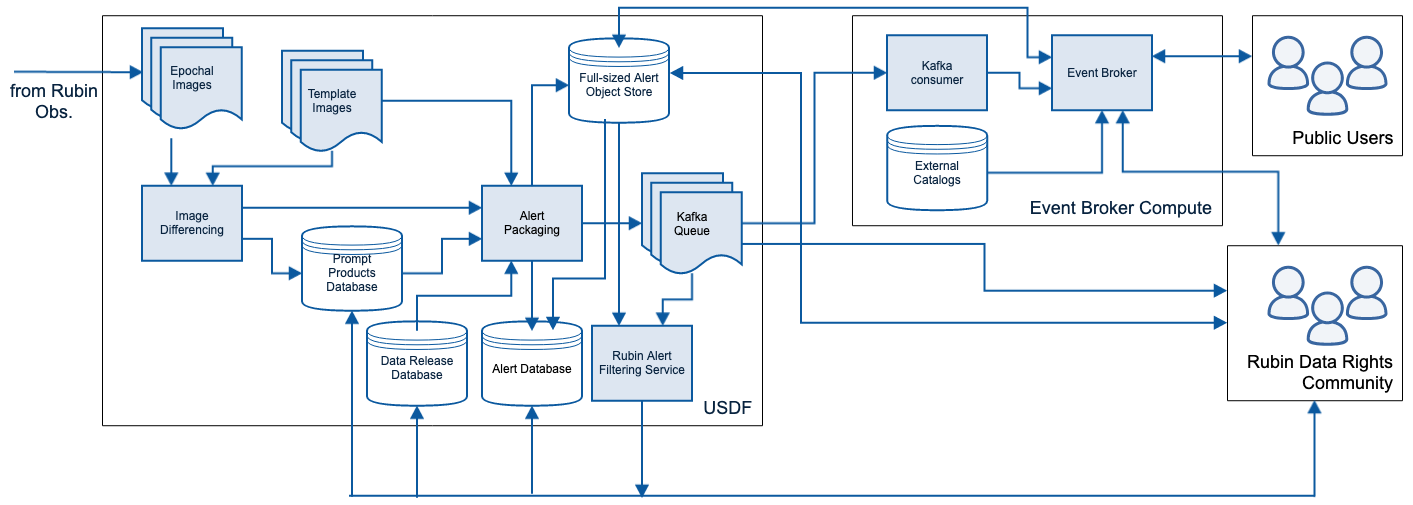
\includegraphics[width=\textwidth]{fig/lightweight_alert_dist.png}
  \caption{Data flow diagram for the proposed lightweight alert system.
  \label{fig:lightweight}}
  \end{centering}
\end{figure}

\section{Technical Implementation}  

% this is ... pretty sparse at the moment
We consider a technical implementation derived from the current baseline as described in 
\citeds{DMTN-093}.
As the Alert Production pipeline runs, it would produce both the full-sized alert packets and their lightweight counterparts, both in Avro format.
The lightweight alerts would be distributed to community brokers and science users using Kafka.
The full-sized alerts would be stored on disk in an object store or other system accessible by HTTP.
Brokers and users would obtain an identifier from lightweight alerts and request the corresponding full-sized alerts via HTTP.

% more about the rate limit implementation?

%  URL for packet retrieval -- longevity
The link to retrieve the full-sized alert must be permanent, even if the full-sized alert is moved.  
This suggests use of an identifier such as a DOI, URI, or IVORN\footnote{\url{https://www.ivoa.net/documents/IVOAIdentifiers/20160523/index.html}}.

\section{Implications for the Alert Filtering Service} \label{sec:alertfiltering}

In the current baseline, Rubin Observatory runs an Alert Filtering Service (AFS) within the Data Facility that allows a limited number of users ($\geq$100 simultaneous\dmreq{0343}\reqparam{numBrokerUsers}) with Data Rights to upload filters and have a limited number of alerts ($\leq$ 20 per visit\reqparam{numBrokerAlerts}) forwarded to them.
In addition to the limited capacity, the AFS restricts the user filters to only operate on the contents of the alert packets themselves.
There is currently no latency requirement for alert delivery through the AFS.

We suggest that the lightweight alert packet design would obviate the scientific need for the AFS, reducing Project scope.
Instead of providing filter code to run on Data Facility services, users with data rights could run filters on their own hardware with a great deal more flexibility.
In particular, users would be free to build filters that crossmatched to external catalogs or realtime streams or performed computationally-intensive fitting or image-processing tasks.
They would be free to choose their own programming language, libraries, and environment.
While the need to implement their own local service would impose additional difficulty relative to a Project-provided AFS, the Project could provide simple tutorial material for a basic implementation.

%\textbf{estimate data rates for 100x20.  20 full-sized alerts per filter had to come out anyway}

One particular advantage of this scheme to users is that within their overall rate limit budget, they could receive more alerts from single visits at cost of higher latency.
The AFS is likely to have had hard limits at 20 full-sized alerts per visit, after which no more would be forwarded.
In contrast, a user wanting many more alerts from a high-priority single visit (say, a Deep Drilling field) could simply request more full-sized alerts over a longer period of time.

Descoping the AFS would reduce on-Project construction and operations effort.

\section{Implications for the Alert Database} \label{sec:alertdb}

The store of full-sized alerts is conceptually quite similar to the ``Alert Database,'' a component of the alert system that is required as a record of all transmitted alerts but that has relatively few other enumerated requirements\dmreq{0094}.
Particularly if flexible identifiers pointing to the full-sized alerts are used, it seems useful to investigate whether the Alert Database and the store of full-sized alerts could be the same system, technically.
This would provide a seamless transition for the user between active and archival alerts.
Users could retrieve full-sized alerts by their URIs, and it would be straightforward to implement additional queries (cone search, time window, etc.) by querying the Prompt Products Database and retrieving the appropriate alert URIs.
It would also be necessary to archive the lightweight alerts, but due to their small size this should not be a large perturbation.

\section{Other Potential Approaches} \label{sec:alerternatives}

Are there other ways to increase the reach of the alert stream in the baseline, full-size alert scenario?
Given the scale of the full-sized alerts, any such approach would still rely on community brokers to provide alert access.
However, the total number of community brokers could be increased by allocating more bandwidth at the Data Facility, by providing a "fan-out" service replicating the alert stream, and/or by relaxing the 60-second latency requirement.


\section{Advantages}

The most significant advantage of this system is that it makes alerts immediately available to a much broader audience.
This was identified by attendees as a major priority from the 2019 Broker Workshop, in preference to a hard selection of a subset of the attending broker teams.
``Alerts on your laptop'' is also an exciting pitch for average scientists and is likely to provide large improvements in science use and uptake of the alert stream, even if users eventually choose to migrate to more full-service brokers.
%  Much wider availability of the alert stream (alerts on your laptop)--a priority from the Broker Workshop; potentially huge improvements in uptake of alert stream
%  more transformative use of the alert stream

We expect improved technical performance, as the the lightweight stream and the full packet archive systems can be designed separately.
Bulk transport and rapid notification workloads tend to have quite different architectures.

%  More effective use of datacenter bandwidth
While we will still meet the 60-second latency requirement, in practice we expect that this design will produce more effective use of the datacenter bandwidth.
In the baseline design all of the alerts must be transmitted to the selected brokers within a relatively narrow window to meet latency requirements.
The system will still be capable of this performance.
However, since brokers will now control retrieval of the full packets, in practice they are likely to spread their queries out in time, smoothing the ``peaky'' nature of the traffic demands and enabling more users to make use of the connection.

This ability to control the flow of the data likely also provides a technical advantage for broker systems in handling the large data volumes.
Within the lightweight stream, brokers will no longer need to stream through all of the bytes of a full alert in order to get to the next one, and they will then be able to fan out retrieval and processing of the full alerts in parallel.
% spencer talk

% Makes it easier to accomodate demand for three cututs/larger cutouts
Some science users have requested more information be included in the alerts---in particular, a third cutout image, and larger cutout images than the DPDD requires.
These further increases to the size of already heavy alerts can be more easily accommodated if the delivery of the full alert payload is decoupled from the realtime notification.

While not a feature of the design presented here, we speculate that users may wish to retrieve only a portion of the full-sized alert---the cutouts, say, or the \DIASource history.
A small service extracting only the relevant alert portion would provide further improvements in bandwidth use.

Finally, the proposed system provides potential improvements in interfacing with the alert filtering service and alert archive, as discussed in \S \ref{sec:alertfiltering} and \S \ref{sec:alertdb}.
%  Opportunity for more seamless transition between alert stream and alert archive

\section{Challenges and Concerns}
%  Two systems, not one (but: may save labor with alertdb/lafs)
Among the technical challenges presented by the hybrid alert design is that it requires the Rubin Observatory project to design and administer two systems (the lightweight stream and the full-size alert retrieval system) rather than one (a full-sized alert stream).
Given the late stage of the construction project it is reasonable to question whether it is prudent to consider such a change.
However, the baseline also requires construction of the alert database and the alert filtering service, and as discussed (\S \ref{sec:alertfiltering}--\ref{sec:alertdb}) the lightweight alerts design may provide some simplifications to those systems.

% Much wider audience for Kafka stream may be technically challenging
In our baseline, only a small number of alert brokers receive the Kafka stream.
While moving to smaller alerts will improve Kafka's performance, distributing a lightweight Kafka stream to a much wider audience may require further attention.
We do not anticipate challenges scaling the Kafka system itself to many consumers, but Kafka is primarily used as a streaming solution \textit{within} organizations, and as of this writing its capabilities for handling many untrusted third-party consumers is less mature.

It will require effort and scientific consensus-building to identify a minimal subset of alert contents for lightweight alerts that maintains its small size but provides the necessary information for efficient filtering.
There will be community demand to repeatedly increase the number of included fields to satisfy individual science cases.

%  Additional broker latency
For the small number of brokers who are allowed to receive the full stream, the additional round-trip to retrieve the full alert packet imposes a small amount of additional latency (In the best case, roughly 200\,msec).
Additionally it requires brokers to re-engineer existing alert retrieval code.
The handful of full-stream brokers may view these as pure costs with no benefit relative to the baseline.
We believe these costs are justified by the gains of being able to distribute the alerts more widely; the modest additional latency is not scientifically significant.
As discussed above, brokers may ultimately find it technically advantageous to be able to have their own systems direct and parallelize the retrieval of the largest volumes of data.

%  Data rights issues
The most pressing concerns are those of data access.
Alert packet contents are world public; this would include both the lightweight alerts and the full-sized alerts.
However, access to databases and services within the Rubin Data Facility is restricted to data-rights holders \citedsp{RDO-013}.
If the same consideration applies here, only users with data rights could subscribe to the lightweight stream and access the full-sized alerts directly\footnote{We do support investigating whether true world-public \textit{access} to the lightweight alerts and full alerts with very low rate limits could be supported.}.
As in the current baseline, users without data rights would rely on community alert brokers to access the public alerts.
Since the lightweight alerts could be much more widely distributed to individual users, this situation would highlight more starkly the distinction between data rights and data access to the (world-public) alerts, which might create confusion or frustration among scientists.

%need for authentication (for data rights, also for rate limits)
Both the lightweight alert stream and the packet retrieval service would require authentication and authorization to confirm data rights and set appropriate rate limits.
Individuals may find rate limits frustrating if their alert retrieval needs don't match their rate limits and may pressure the project for greater access rather than adopting their workflow to use a community broker.
% is this different than the baseline?

The lightweight alerts contain a URI that points to the corresponding full alert packet.
If a user without data rights is unable to access the packet at that location, having a copy of the world-public lightweight alert is not very useful.
While community brokers are responsible for providing public access to alerts even in the baseline, they would need to provide their own additional URL or URI pointing to a publicly-accessible copy of the full alert, which could create confusion.
From a pure user-experience perspective this suggests making access to the full alerts world-public, even if the rate limits for non-data-rights holders are extremely low.

Referential integrity of the lightweight and full alerts could be hard to maintain. 
Perfect synchronization of the data and notification systems is probably impossible, which could impact users' ability to rapidly retrieve the full alerts.

Because brokers must now actively retrieve the full alert packets, this inhibits architectures where the brokers provide only stateless real-time filtering or forwarding of alerts.
This pattern does not appear common among the precursor brokers operating on ZTF, however.

A broad concern is whether lightweight alerts are beneficial to community brokers.
We believe from a technical standpoint that brokers will benefit from being able to retrieve the full-size alerts when desired and in parallel, rather than being forced to stream through each alert to get to the next one.
But for the top five selected brokers this benefit is probably not large.
The greater advantage is to community brokers that might not otherwise be able to access the full alert stream, either directly from the project or from an ``upstream'' community broker.
It is difficult to quantify this impact at present; the SAC's evaluation of the full broker proposals will be useful here.
And there are other alternatives for increasing the number of community brokers served (\S \ref{sec:alerternatives}).

% Is this just a broker function?
As discussed in \S \ref{sec:alertfiltering}, the biggest beneficiaries of the lightweight alert stream are likely to be single science users or small groups, who can now receive the complete lightweight alert stream and perform more sophisticated analysis than is possible with the baselined Alert Filtering Service.
It may be argued that filtering and/or redistribution of alerts with fewer contents can or will be performed by the brokers themselves, and Rubin's efforts are thus duplicative (and may even hinder broker teams' ability to obtain funding).
We expect that community brokers will be the dominant way that users will access LSST alerts thanks to their scale, ease of use, and integration with other facilities.
However, the Project aims to maximize the scientific return from the survey; making lightweight alerts broadly available will not hinder the use of community brokers and are likely to enable fresh new ideas and applications.

%  VO-first


\appendix

\section{Possible lightweight alert packet contents} \label{sec:lightweight_contents}

Table \ref{tab:lightweight_alert} provides a list of candidate fields that could be included in a lightweight alert and enable substantial pre-filtering by science users before they needed to retrieve the full alert packets corresponding to a subset of alerts.

\begin{table}
  \begin{centering}
  \begin{tabular}{|l|r|r|}
    \hline
Field	& Type &	bytes \\
\hline
alert contents URI &	varchar(80)	& 80 \\
diaSourceId	&  unit64	& 8 \\
filterName &  	unit8	& 1 \\
programID	& unit16	& 2 \\
diaObjectId	& unit64 &	8 \\
ssObjectId &	unit64 &	8 \\
midPointTai &	double &	8 \\
ra &	double & 	8 \\
dec &	double & 	8 \\
psFlux &	float	& 4 \\
psFluxErr &	float	& 4 \\
totFlux	 & float &	4 \\
totFluxErr & 	float	& 4 \\
trailLength	& float	& 4 \\
extendedness & 	float & 	4 \\
spuriousness &	float	& 4 \\
number of previous detections	& int16	& 2 \\
time of most recent observation & 	double & 	8 \\
totFluxMean	& float	& 4 \\
totFluxSigma & 	float	& 4 \\
distance to nearest star & 	float	& 4 \\
distance to nearest galaxy	& float	& 4 \\
parallax/PM	& 3 floats &	9 \\
other timeseries or SSObject features & float & TBD \\
\hline
  \end{tabular}
  \caption{A potential set of fields for a lightweight alert packet of $\sim$200 bytes. \label{tab:lightweight_alert}}
\end{centering}
\end{table}
		

% Include all the relevant bib files.
% https://lsst-texmf.lsst.io/lsstdoc.html#bibliographies
\section{References} \label{sec:bib}
\renewcommand{\refname}{} % Suppress default Bibliography section
\bibliography{local,lsst,lsst-dm,refs_ads,refs,books}

% Make sure lsst-texmf/bin/generateAcronyms.py is in your path
\section{Acronyms} \label{sec:acronyms}
\addtocounter{table}{-1}
\begin{longtable}{p{0.145\textwidth}p{0.8\textwidth}}\hline
\textbf{Acronym} & \textbf{Description}  \\\hline

 &  \\\hline
DM & Data Management \\\hline
DMTN & DM Technical Note \\\hline
DOI & Digital Object Identifier \\\hline
DPDD & Data Product Definition Document \\\hline
GB & Gigabyte \\\hline
HTTP & HyperText Transfer Protocol \\\hline
KB & KiloByte \\\hline
LSST & Legacy Survey of Space and Time (formerly Large Synoptic Survey Telescope) \\\hline
NEO & Near-Earth Object \\\hline
PM & Project Manager \\\hline
RDO & Rubin Directors Office \\\hline
SAC & Science Advisory Committee \\\hline
TBD & To Be Defined (Determined) \\\hline
URL & Universal Resource Locator \\\hline
ZTF & Zwicky Transient Facility \\\hline
kbps & kilobits per second \\\hline
\end{longtable}

% If you want glossary uncomment below -- comment out the two lines above
%\printglossaries





\end{document}
